\documentclass[a4paper, 10.5pt, twoside]{jreport}

% include
\usepackage{gra_yasuda}
\usepackage{lscape}
\usepackage{graphicx}
\usepackage{here}
\usepackage{color}
\usepackage{amsmath}
\usepackage{subfig}
\usepackage{tascmac}
\usepackage{url}
\usepackage{ascmac}
\usepackage{booktabs}
\usepackage{otf}
\usepackage{comment}



%タイトル
\title{心理的効果を用いた人間とエージェントの繰り返し交渉戦略}
\etitle{Repetitive negotiation strategy of human and agent \\ using psychological effect}

%名前
\author{松下 昌悟}
\eauthor{Shogo MATSUSHITA}

%入学年度
\enteryear{2017}
%卒業年度
\graduateyear{2018}

%学籍番号
\studentnumber{17268508}

%提出日
\date{平成30年1月31日}

\begin{document}

%ここで行ピッチを指定
%フォントを変えるとサイズがリセットされてしまうので注意
\setlength{\baselineskip}{8truemm}


%ここから内容

% Chapter 5
\chapter{評価実験}\label{cha:5}

\section{目的と概要}
提案手法の有用性を示すことを目的として人間とエージェントで交渉を行う.
被験者は提案手法の戦略を適用した8つのエージェントにベースラインであるNotNotエージェントを加えた計9種類のエージェント全てと交渉を行う.
本実験では,提案手法の戦略を適用したエージェントの個人効用が高いほど良い戦略であると評価する.

\section{実験設定}
評価実験で用いるドメインは予備実験で用いたドメイン(表\ref{tab:pre_domain})と同一のものである.


\section{実験結果と考察}
エージェントと被験者の個人効用の差分とその分散,エージェントと被験者の社会的余剰の平均とその分散,エージェントの交渉決裂率の平均とその分散をそれぞれ図\ref{fig:pre_util},図\ref{fig:pre_social},図\ref{fig:pre_broken}に示す.

\begin{figure}[h]
  \centering
  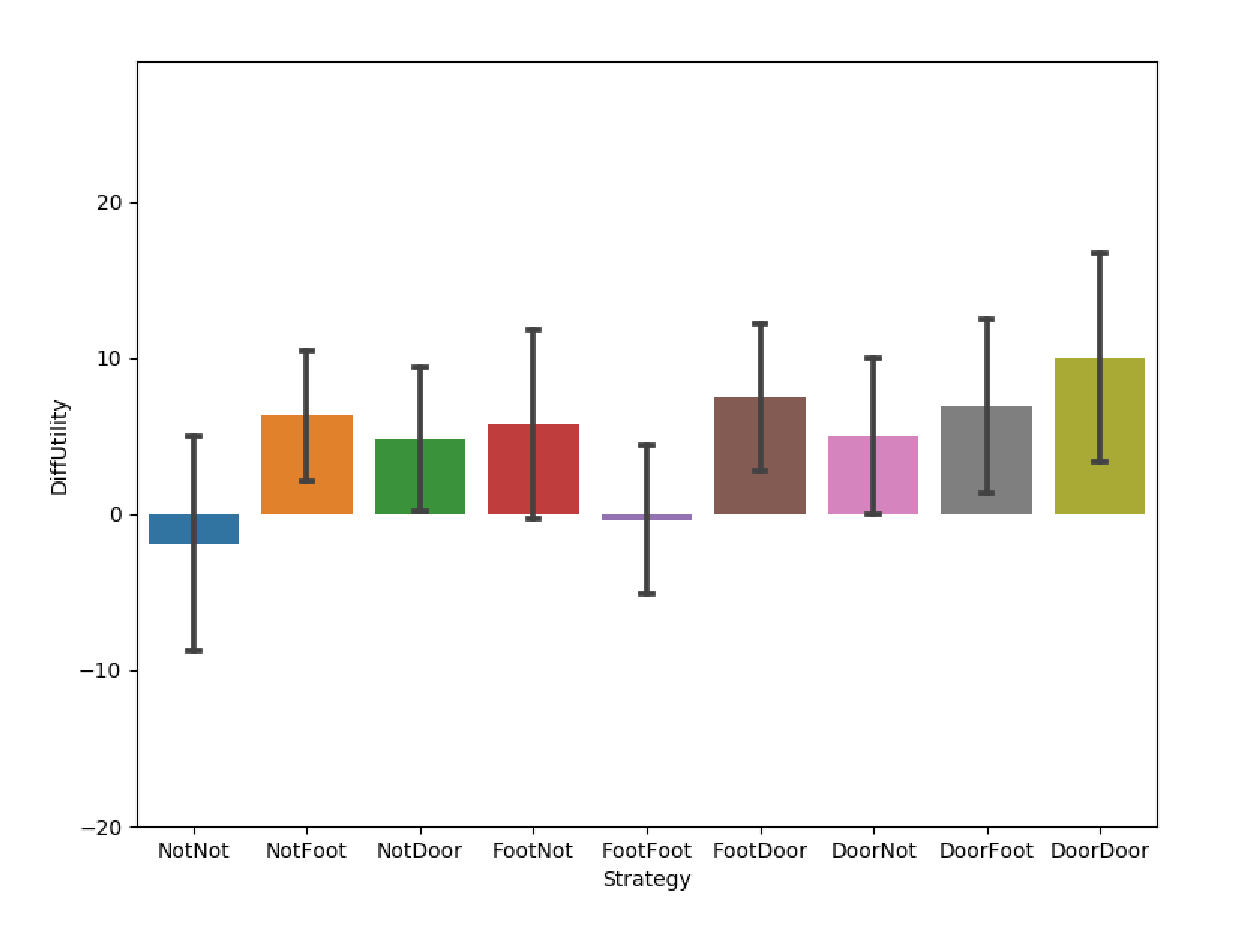
\includegraphics[width=12truecm]{image/result_utility_diff.eps}
  \caption{エージェントと被験者の得られた効用の差分}
  \label{fig:res_util_diff}
\end{figure}

\begin{figure}[h]
  \centering
  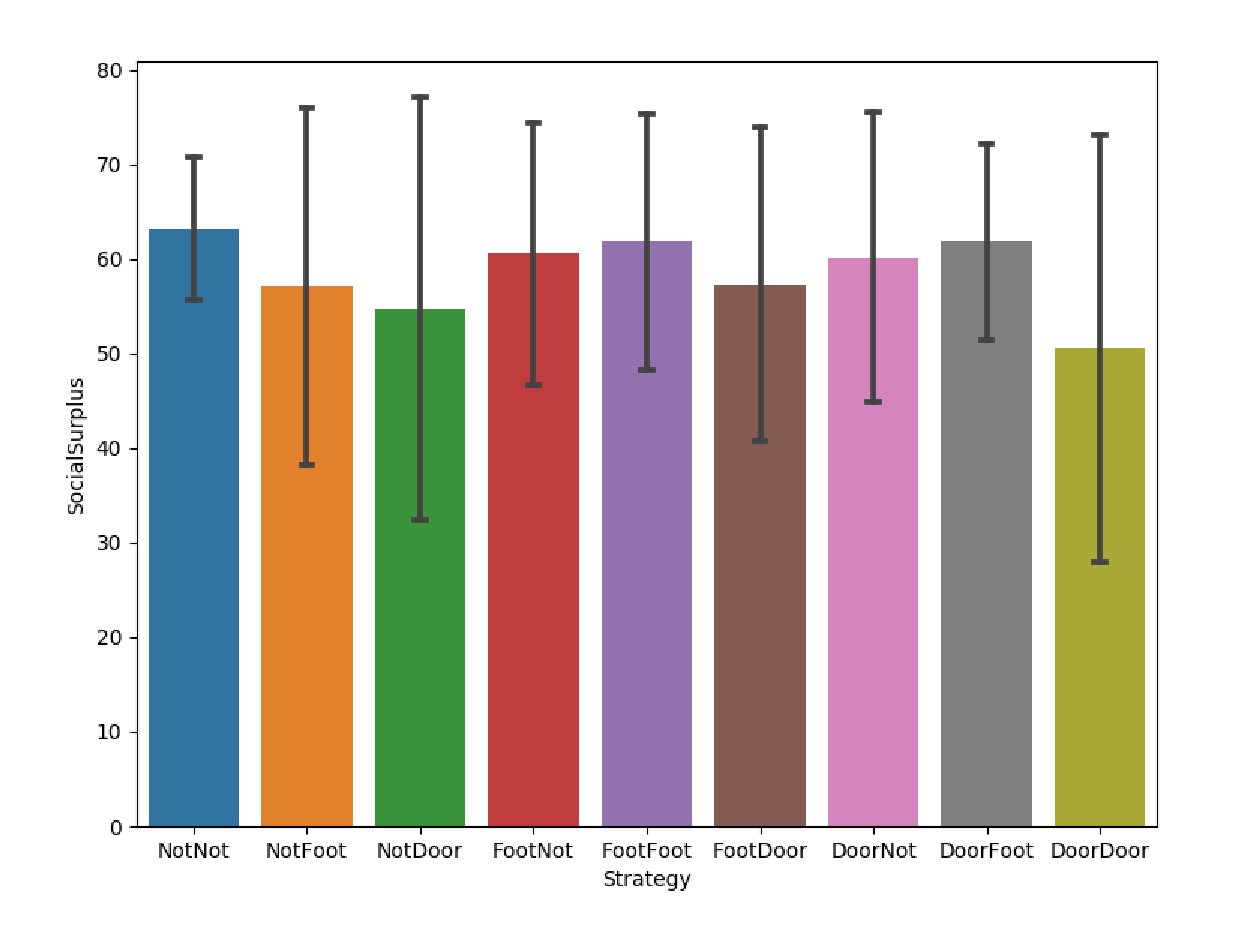
\includegraphics[width=12truecm]{image/result_social_surplus.eps}
  \caption{エージェントと被験者の社会的余剰}
  \label{fig:res_social}
\end{figure}

\begin{figure}[h]
  \centering
  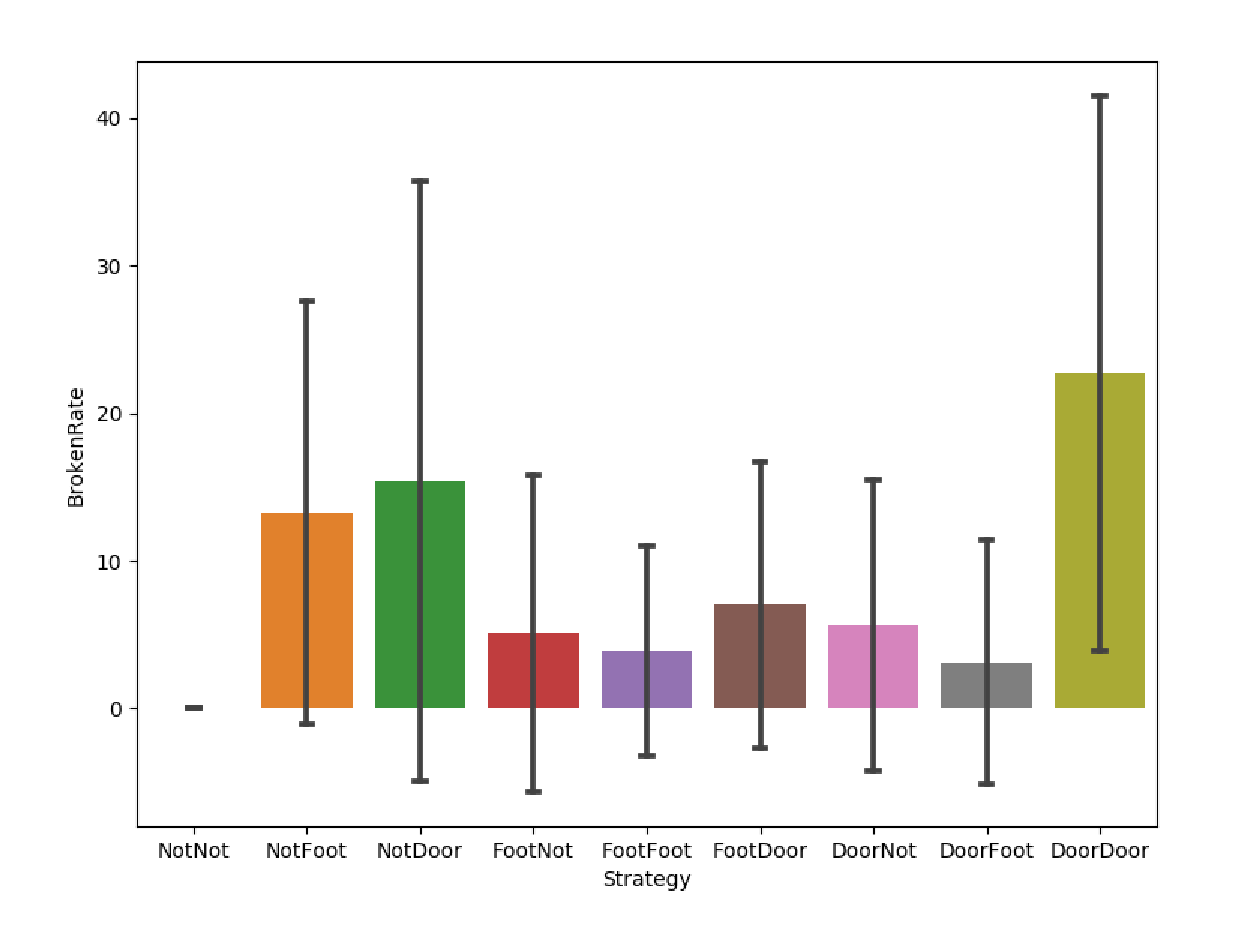
\includegraphics[width=12truecm]{image/result_broken_rate.eps}
  \caption{エージェントの交渉決裂率}
  \label{fig:res_broken}
\end{figure}

%内容ここまで

\chapter*{謝辞}
本論文を執筆するにあたり,多数の方々からご指導・ご協力いただきましたことを,心より御礼申し上げます.

指導教員である藤田桂英准教授には,研究の機会を与えていただき,研究の方針に関する助言や発表練習等の
多大なるご指導や助言をいただきましたことを深く感謝いたします.

研究に関する知識のご教示に加えて,本実験の準備を行うにあたってWEBサーバを構築する際にお力添えいただいた松根鷹生様に深く感謝申し上げます.
また,藤田桂英研究室の皆様には研究に必要な知識や意見等をいただいたことを心より感謝いたします.

本実験を行うにあたってお忙しい中ご協力いただいた同期の編入生の方々,および安井貴規様がいなければ本論文は完成に至りませんでした.
心より御礼申し上げます.

最後に,様々な面で私を支えていただいた家族に,心より感謝いたします.ありがとうございました.

\bibliographystyle{plain}
\bibliography{reference}


\begin{comment}
%付録で発表論文をつけてアピールだ!!

\renewcommand{\bibname}{付録 発表論文一覧}
%\chapter{発表論文一覧}

\begin{thebibliography}{99}
\item S. Kakimoto and K. Fujita. 二者間複数論点交渉問題におけるパレートフロント推定手法の提案. Joint Agent Workshop and Symposium, 2014.
\item S. Kakimoto and K. Fujita. Estimating Pareto Fronts using Interdependency between Issues for Bilateral Multi-issue Closed Nonlinear Negotiations. Applications Knowledge and Service Technology for Life, Environment, and Sustainability workshop(KASTLES),2014.
\item S. Kakimoto and K. Fujita. 二者間非線形交渉問題におけるパレートフロント推定を利用した自動交渉エージェントの設計と評価. 情報処理学会 第177回 知能システム研究会, 2014.

\end{thebibliography}

\end{comment}

\end{document}

